
\documentclass{plot-softwaremanual}

% Packages used in this example
\usepackage{graphicx}  % for including images
\usepackage{microtype} % for typographical enhancements
\usepackage{minted}    % for code listings
\usepackage{amsmath}   % for equations and mathematics

\usepackage{pgfplots}
\setminted{style=friendly,fontsize=\small}
\usepackage{hyperref}  % for hyperlinks
\usepackage[a4paper,top=4.2cm,bottom=4.2cm,left=3.5cm,right=3.5cm]{geometry} % for setting page size and margins


% Frontmatter data; appears on title page
\title{Software Tools - \texttt{\LaTeX}  \vspace{}Assignment \\Matlab - Plots}

\author{{\textcolor{grey}{\btt Sonam Bharti}} \\
      {\ttfamily 2021pcs2040@iitjammu.ac.in}\hspace{}}
\softwarelogo{
\includegraphics[width=15cm]{./Images/IIT_JAMMU_LOGO.png}}

\begin{document}

\maketitle

\tableofcontents

\newpage

\section{Introduction}
\subsection{Definition}
textcolor{Emerald}{\btt Definition}
  \begin{enumerate}
     \item To plot the graph of a function, you need to take the following steps $-$
            \begin{enumerate}
                    \item Define the function, {\textbf{y = f(x)}}
                    \item Call the {\textbf{plot}} command, as {\textbf{plot(x,y)}}
            \end{enumerate}
            
            \item {\textbf{\Small{Example:}}} Plot the function 
            $$y = x^2 - 10x + 15 $$\\
            for the values of x between 0 and 10.\\\pause
            \centering{x = 0:1:10  \hspace{}  {\textcolor{blue}{   or  }} linspace(0,10,11)} 
  \end{enumerate}


\subsection{Example}

Code:\\

\vspace{\height=10}
\hspace{\height=3}

\noindent\fbox{
    \parbox{\textwidth}{
        x = 0:1:10;\\
        $y = x.^2-10*x+5$\\
        plot(x,y)\\
        grid on\\
    }
}


\vspace{\height=25}
\hvspace{\height=3}
   \centering 
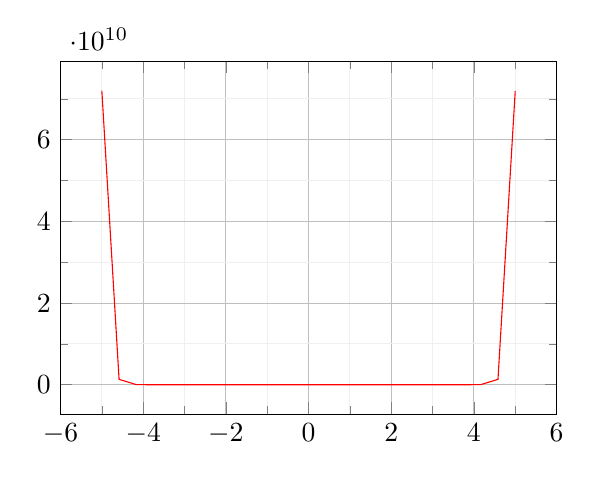
\begin{tikzpicture}
    \begin{axis}[
            grid = both,
            major grid style = {lightgray},
            minor grid style = {lightgray!25},
            minor tick num = 1,
            width = 0.65\textwidth,
            height = 0.5\textwidth,
            ]
        \addplot[
            x=0:1:10
            smooth,
            thin,
            red] {exp (x^2)-10*x + 5 };
       
    \end{axis}
\end{tikzpicture}
\label{Plot 1: Matlab Plot Example}



\section{Matlab Plots}

\subsection{Terms}

\texttt {Terms generally used in Matlab plotting are}...\\
    \begin{enumerate}
    
    \item {\textbf {CLF:}} clf deletes all children of the current figure that have visible handles.
    
    \item {\textbf {clf(fig):}} It deletes all children of the specified figure that have visible handles.
    
    \item {\textbf {figure:}} It creates a new figure window using default property values. The resulting figure is the current figure.
    
    \item {\textbf {figure(n):}} It  finds a figure in which the Number property is equal to n, and makes it the current figure. If no figure exists with that property value, MATLAB® creates a new figure and sets its Number property to n.
    
    \item {\textbf {figure(Name, Value):}} It modifies properties of the figure using one or more name-value pair arguments. For example, figure('Color','white') sets the background color to white.
    
    
    \item {\textbf {hold on:}} It retains plots in the current axes so that new plots added to the axes do not delete existing plots. 
    
    \item {\textbf {hold off:}} It sets the hold state to off so that new plots added to the axes clear existing plots and reset all axes properties. 
    
    \item {\textbf {grid on:}} This command allows us to put the grid lines on the graph.
    
    \item {\textbf {grid off:}} This command allows us to remove the grid lines on the graph.
    
    \item {\textbf {title:}} This command allows us to put a title on the graph.
    
    \item {\textbf {xlabel}} and {\textbf {ylabel:}} These commands generate labels along x-axis and y-axis.
    
 
    
    \item {\textbf {axis equal:}} This command allows generating the plot with the same scale factors and the spaces on both axes.
    
    \item {\textbf {axis square:}} This command generates a square plot.
    \item {\textbf {legend:}} Legend function is used to add descriptive labels to our plots.
    
    \item {\textbf{plot:}} It plots the curve defined by the function y = f(x) over the default interval [-5 5] for x.
    \item {\textbf{bar:}} It creates a bar graph with one bar for each element in y. If y is an m-by-n matrix, then bar creates m groups of n bars.
    
    \item {\textbf{scatter:}} It creates a scatter plot with circular markers at the locations specified by the vectors x and y.

  \end{enumerate}
\hspace{}
 
\subsection{Plot Types}

\vspace{\height=10}
\hspace{\height=3}

\texttt{There are many types of plots\footnote{Reference of plot types are taken from 
\doclink{\url{https://in.mathworks.com/help/matlab/creating_plots/types-of-matlab-plots.html}}{ Mathworks.}} in Matlab. Some of them are....}

\vspace{\height=10}
\hspace{\height=3}

\begin{figure}[hbp]
    \centering
    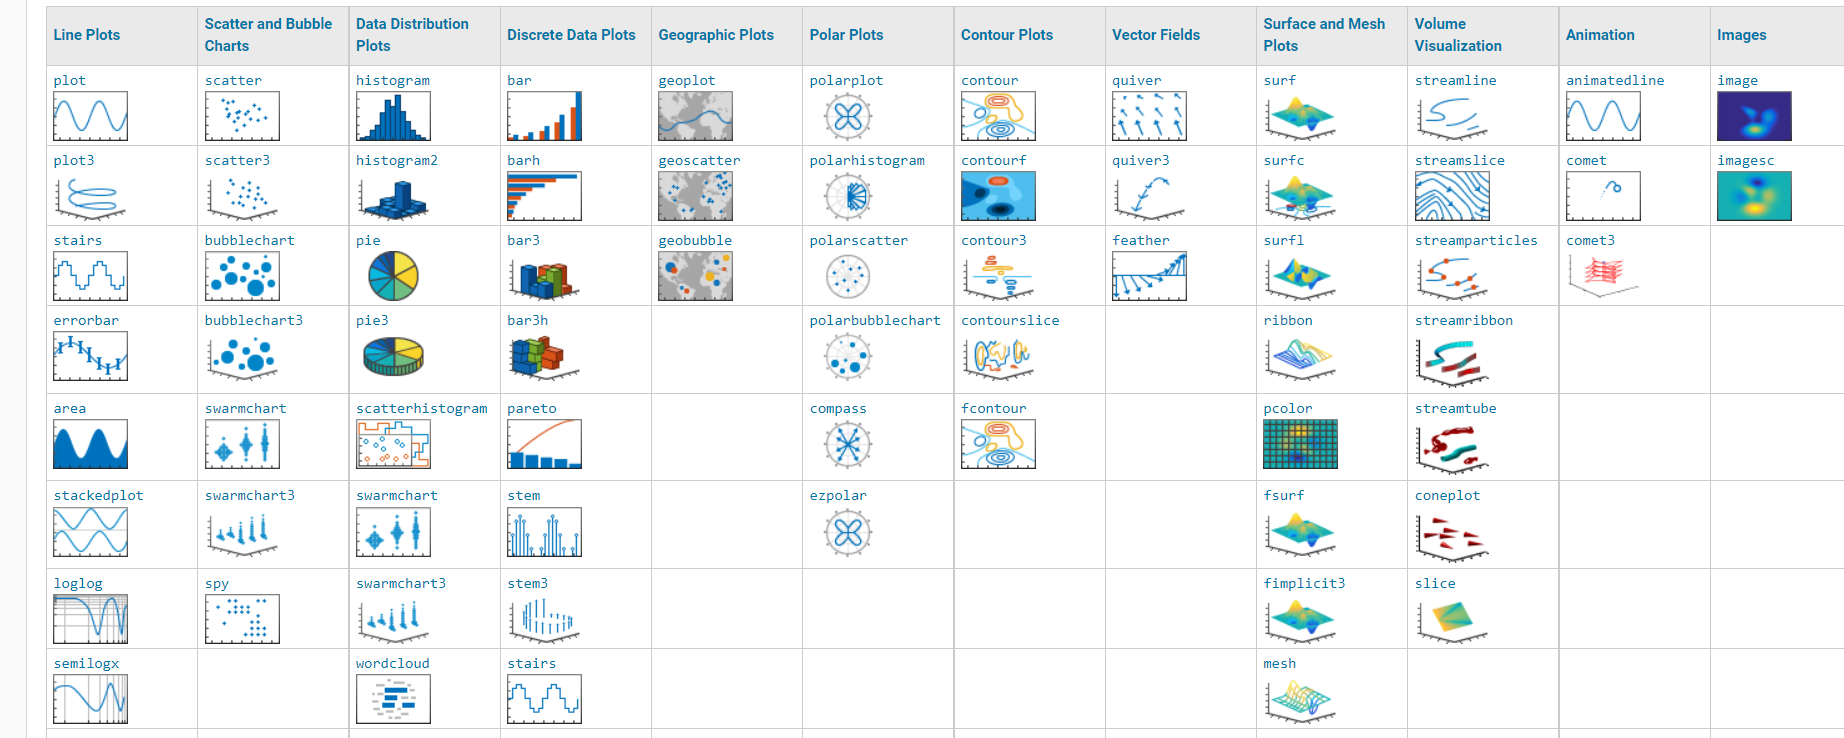
\includegraphics[width=15cm, height=8cm]{Images/plot-types.png}
    \caption{\label{fig:my_label}Plot Types in Matlab}
    
\end{figure}

\newpage
\begin{block}
\texttt{The main types of plot which we generally talk about are:}
  \begin{enumerate}
    \item {\tt Line Plots}
    \item {\tt Bar Graph}
    \item {\tt Histogram}
    \item {\tt 2D Scatter}
    \item {\tt Pie Chart}
    \item {\tt Area}
    \item {\tt Sinusoidal}
    \item {\tt Log, Exponential}
    \item {\tt Geo-plot}
    \item {\tt Geo-scatter}
    
  \end{enumerate}
\end{block}

%% \newpage

\section{Plot Types Example}
\subsection{Single Plot}
\subsubsection{Sinudoidal}
Code:\\
\vspace{}
\hspace{}
\noindent\fbox{
    \parbox{\textwidth}{
        $x = 0:pi/100:2*pi$\\
        $y = sin(x)$\\
        plot(x,y)\\
        grid on\\
        legend('simple plot')\\
    }
}

\vspace{\height=25}
\hspace{\height=3}
   \centering 
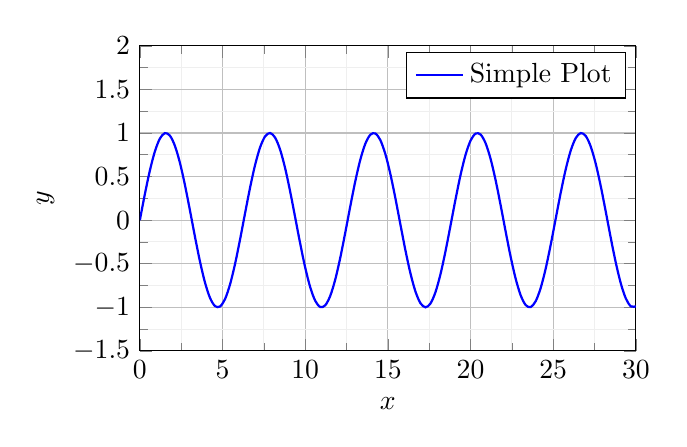
\begin{tikzpicture}
    \begin{axis}[
            xmin = 0, xmax = 30,
            ymin = -1.5, ymax = 2.0,
            xtick distance = 5,
            ytick distance = 0.5,
            grid = both,
            minor tick num = 1,
            major grid style = {lightgray},
            minor grid style = {lightgray!25},
            width = 0.65\textwidth,
            height = 0.45\textwidth,
            xlabel = {$x$},
            ylabel = {$y$},
            legend cell align = {left},
            ]
        \addplot[
                domain = 0:30,
                samples = 100,
                smooth,
                thick,
                blue,
            ] {sin(deg(x))};
        \legend{Simple Plot}
    \end{axis}
\end{tikzpicture}\\
\caption{\label{fig:plot} \textbf{Graph:} Simple plot }

\subsubsection{Bar Graph}
Code:\\
\hspace{}
\vspace{}
\noindent\fbox{
    \parbox{\textwidth}{
        clf\\
        x = 1:5\\
        y = [2 11 6 9 3]\\
        figure(1)\\
        bar(x,y)\\
        grid on\\
        legend('bar graph')\\
    }
}

\vspace{\height=15}
\hspace{\height=3}
\centering 
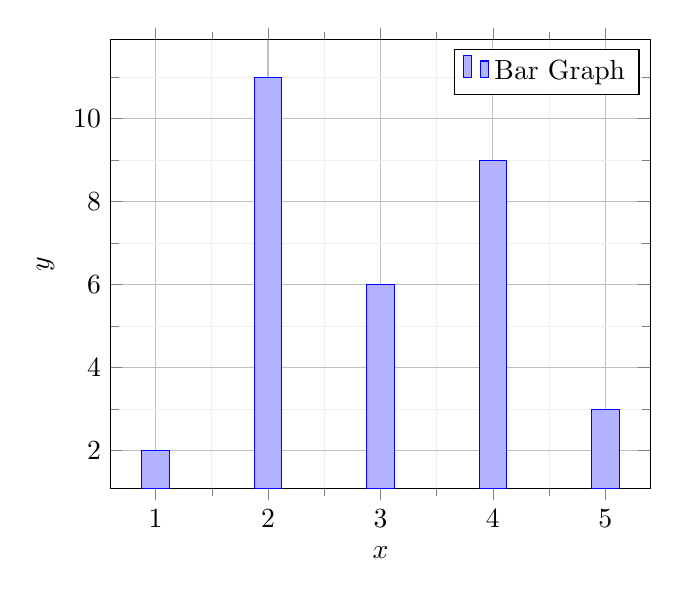
\begin{tikzpicture}
    \begin{axis}[
            ybar,
            grid = both,
            minor tick num = 1,
            major grid style = {lightgray},
            minor grid style = {lightgray!25},
            xlabel = {$x$},
            ylabel = {$y$},
            legend cell align = {left},
            ]
        \addplot coordinates{
            (1,2)
            (2,11)
            (3,6)
            (4,9)
            (5,3)};
        \legend{Bar Graph}
        
    \end{axis}
\end{tikzpicture}\\
\caption{\label{fig:plot} \textbf{Graph:} Bar Graph}

\subsection{Multiple Plot}

Code:\\

\vspace{}
\hspace{}
\noindent\fbox{
    \parbox{\textwidth}{
        clf\\
        $x = linspace(-2*pi,2*pi)$\\
        $y1 = (-x/10) * cos(x) + sin(x)/10 $\\
        $y2 = cos(x)$\\
       
        figure(2)\\
        plot(x,y1,'-')\\
        
        hold on\\
        plot(x,y2,'--')\\
        grid on\\
        legend('y1','y2')
    }
}



\vspace{\height=25}
\hspace{\height=3}
   \centering 
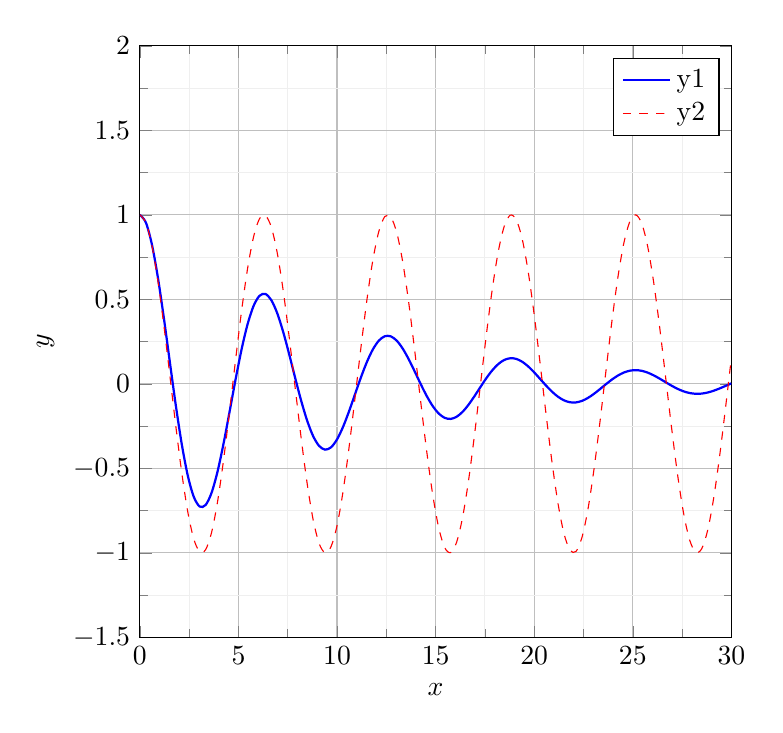
\begin{tikzpicture}
    \begin{axis}[
            xmin = 0, xmax = 30,
            ymin = -1.5, ymax = 2.0,
            xtick distance = 5,
            ytick distance = 0.5,
            grid = both,
            minor tick num = 1,
            major grid style = {lightgray},
            minor grid style = {lightgray!25},
            width = 0.75\textwidth,
            height = 0.75\textwidth,
            xlabel = {$x$},
            ylabel = {$y$},
            legend cell align = {left},
            ]
        \addplot[
                domain = 0:30,
                samples = 100,
                smooth,
                thick,
                blue,
            ] {exp(-x/10)*( cos(deg(x)) + sin(deg(x))/10 )};
            
        \addplot[
                domain = 0:30,
                samples = 100,
                smooth,
                thin,
                red,
                dashed
            ] {cos(deg(x))};
        \legend{y1,y2}
    \end{axis}
\end{tikzpicture}\\
\caption{\label{fig:plot} \textbf{Graph:} Multiple plot Graph}

\newpage

\subsection{Scatter Plot}

Code:\\
\vspace{}
\hspace{}
\noindent\fbox{
    \parbox{\textwidth}{
        clf\\
        x = 1:5\\
        y1 = [2 11 6 9 3]\\
        y2 = [4 5 8 6 2]\\
       
        figure(2)\\
        plot(x,y1,'x')\\
        
        hold on\\
        plot(x,y2,'o')\\
        grid on\\
        legend('y1','y2')\\
    }
}


\vspace{\height=25}
\hspace{\height=3}
   \centering 
   \pgfplotstableread{multiple_functions.dat}{\table}
\begin{tikzpicture}
    \begin{axis}[
            xmin = 0, xmax = 6,
            ymin = 0, ymax = 15,
            xtick distance = 0.5,
            ytick distance = 2,
            grid = both,
            minor tick num = 1,
            major grid style = {lightgray},
            minor grid style = {lightgray!25},
            width = 0.75\textwidth,
            height = 0.65\textwidth,
            xlabel = {$x$},
            ylabel = {$y$},
            legend cell align = {left},
            ]
        \addplot[blue, only marks, mark = x] table [x = {x}, y = {y1}] {\table};
            
            \addplot[red, only marks, mark = o, mark size = 3pt]
                table [x = {x}, y = {y2}] {\table};
        \legend{Plot with 'x' mark,
                Plot with 'o' mark}
    \end{axis}
\end{tikzpicture}\\
\caption{\label{fig:plot} \textbf{Graph:} Scatter plot Graph}
\newpage

\section{References}
\begin{block}{Reference}
 \begin{enumerate}

     \item Tutorialspoint \- MATLAB Tutorial \\ \docklink{\url{https://www.tutorialspoint.com/matlab/index.htm}}
     \item MathWorks Documentation \\
     \docklink{\url{https://in.mathworks.com/help/matlab/ref/plot.html}}
 \end{enumerate}

\end{document}
